\subsection{ECOD}

В марте 2022 года в работе \cite{ECOD} был показан простой, но эффективный алгоритм ECOD (Empirical-Cumulative-distribution-based Outlier Detection), который был вдохновлен тем фактом, что аномалии часто являются «редкими событиями», которые появляются на краях распределения. Данный подход имеет ряд важнейших особенностей, которые стоит отметить:

\begin{itemize}[leftmargin=0pt,itemindent=4.6em]
    \item[$\bullet$] простота понимания и интерпретации метода;
    \item[$\bullet$] отсутствие гиперпараметров, что может быть важно в контексте обнаружения аномалий: их часто может быть сложно корректно настроить, поскольку аномальные экземпляры редки и их не всегда просто получить;
    \item[$\bullet$] в данном методе временная сложность линейно зависит от размера входных данных и числа измерений.
\end{itemize}

ECOD использует информацию о распределении данных, чтобы определить, где данные менее вероятны и, следовательно, более вероятны выбросы. В частности, ECOD оценивает \cite{Replace-Outlier-Detection-with-ECOD} эмпирическую кумулятивную функцию распределения ECDF (см. рисунок \ref{fig:ecdf}) для каждой переменной отдельно.

\begin{figure}
  \centering
  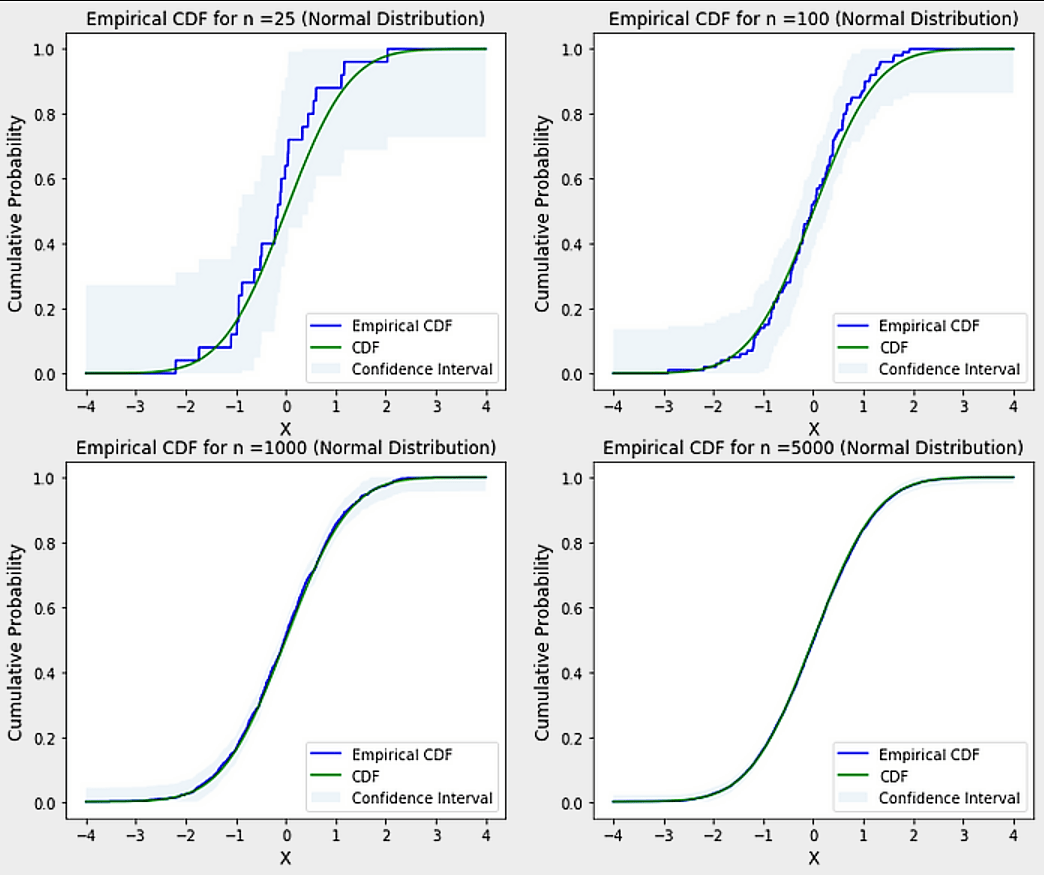
\includegraphics[scale=0.3]{inc/images/ecdf.png}
  \caption{Примеры ECDF для разного объёма выборки нормального распределения \cite{Replace-Outlier-Detection-with-ECOD}}
  \label{fig:ecdf}
\end{figure}

Идеальным вариантом здесь было бы применить объединенный ECDF ко всем переменным; однако это слишком дорого с точки зрения вычислений (скорость сходимости при оценке совместного CDF замедляется по мере увеличения числа переменных). Таким образом, ECOD делает упрощающее предположение о том, что переменные статистически независимы. Но даже с учетом этого предположения ECOD работает довольно хорошо.

Рассмотрим, как работает обучение в данном методе. Пусть на вход поданы данные $X = \{X_i\}_{i=1}^n \in \mathbb{R}^{(n \times d)}$  с $n$ выборками и $d$ признаками. Обозначим $X_i^{(j)}$  значение $j$-го признака для $i$-го экземпляра. Тогда для того, чтобы определить, является ли экземпляр $X_i$  аномалией, необходимо рассчитать 3 вероятностные величины на <<хвостах>> (tails) распределений по формулам (\ref{O_left_def}), (\ref{O_right_def}) и (\ref{O_auto_def}).

\begin{equation}\label{O_left_def}
    O_{left}(X_i)= - \sum\limits_{j=1}^d \log \left[ECDF_{left}^{(j)} (X_i^{(j)} )\right],
\end{equation}
\begin{equation}\label{O_right_def}
    O_{right}(X_i)= - \sum\limits_{j=1}^d \log \left[ECDF_{right}^{(j)} (X_i^{(j)} )\right],
\end{equation}
\begin{equation}\label{O_auto_def}
    O_{auto}(X_i)= \begin{cases}
         - \sum\limits_{j=1}^d \log \left[ECDF_{left}^{(j)} (X_i^{(j)} )\right], &\ \text{если } \gamma_j < 0, \\
         - \sum\limits_{j=1}^d \log \left[ECDF_{right}^{(j)} (X_i^{(j)} )\right], &\ \text{иначе}, \\ 
    \end{cases}
\end{equation}
где $\gamma_j$  – коэффициент асимметрии (skewness) выборки для $j$-го распределения признака (для одной переменной нахождение в левом хвосте распределения вероятностей может быть более аномальным, чем для другой), который, в свою очередь, определяется соотношением (\ref{skewness_coff_def}).
\begin{equation}\label{skewness_coff_def}
    \gamma_j  =  \dfrac{\dfrac{1}{n} \sum\limits_{i = 1}^n \left(X_i^{(j)} - \overline{X^{(j)}}\right)^3}
                       {\left[\dfrac{1}{n-1} \sum\limits_{i = 1}^n \left(X_i^{(j)} - \overline{X^{(j)}}\right)^2 \right]^{^3/_2}}.
\end{equation}

Одно из преимуществ использования отрицательных логарифмов вероятностей заключается в том, что более низкая вероятность преобразуется в более высокое отрицательное логарифмическое значение. Таким образом, редкие элементы с низкой вероятностью получают более высокие оценки аномалий. Тогда результирующую оценку аномальности экземпляра $X_i$ определяется соотношением (\ref{O_def}).

\begin{equation}\label{O_def}
    O(X_i) = \max{ \left\{ O_{left}(X_i),\ O_{right}(X_i),\ O_{auto}(X_i) \right\} } 
\end{equation}


На рисунке \ref{fig:ecod-demo} показано, как комплексный подход к оценке и корректировка асимметрии на основе $\gamma_j$  даёт возможность значительно улучшить результаты в выявлении аномалий в данных. Предложенный метод является эффективным, быстрым и масштабируемым алгоритмом обнаружения аномалий в данных.

\begin{figure}
  \centering
  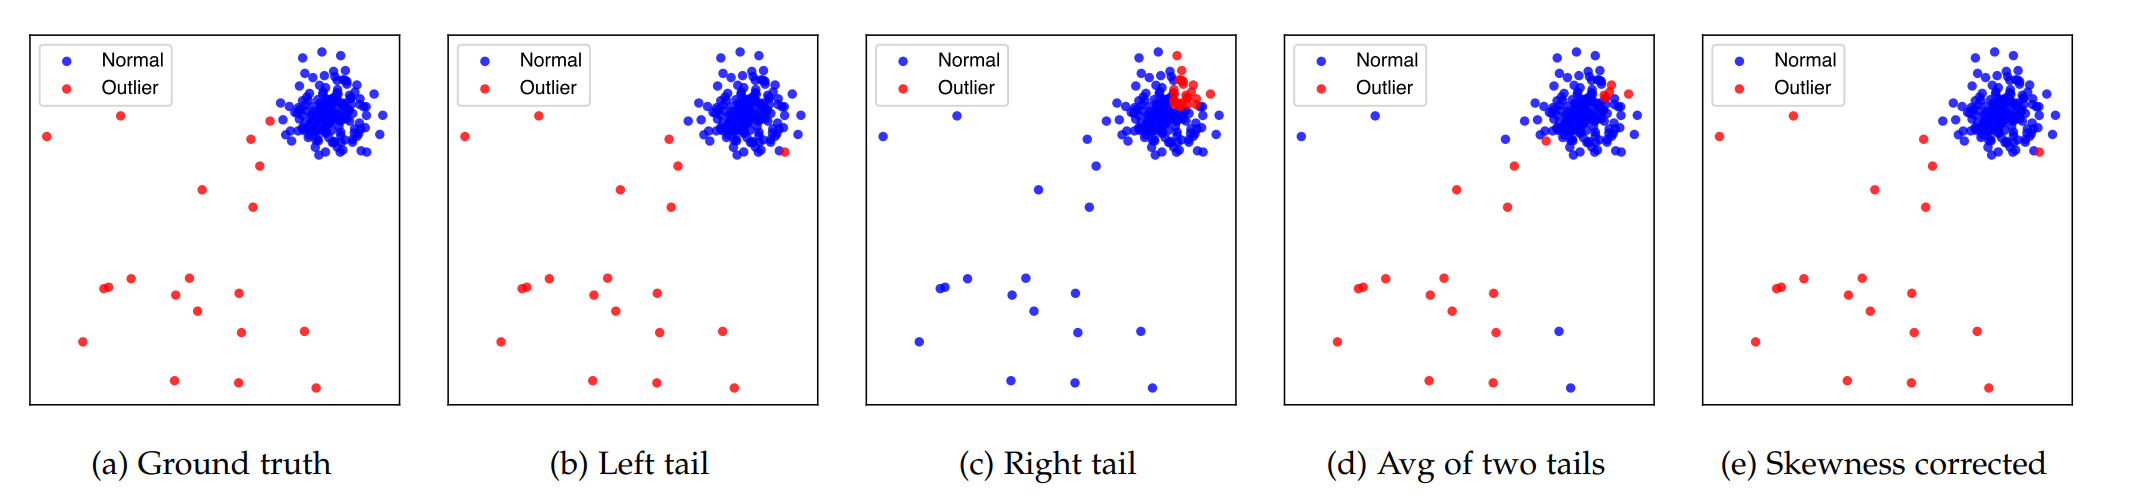
\includegraphics[scale=0.22]{inc/images/ecod-demo.png}
  \caption{Демонстрация влияния «хвостовых вероятностей» и корректировки асимметрии на выявление аномалий \cite{ECOD}}
  \label{fig:ecod-demo}
\end{figure}
